\begin{frame}{Thực nghiệm - Phân loại cấu hình}
  \begin{figure}
    \centering
    \subfloat[Lớp C]{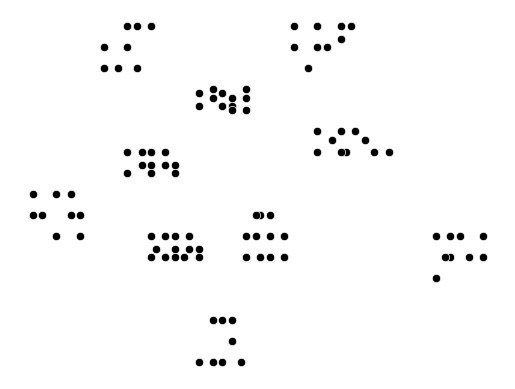
\includegraphics[width=0.3\linewidth]{figures/cls_c.png}}\quad
    \subfloat[Lớp R]{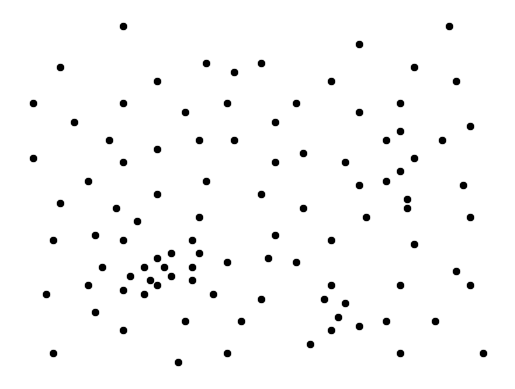
\includegraphics[width=0.3\linewidth]{figures/cls_r.png}}\quad
    \subfloat[Lớp RC]{
\includegraphics[width=0.3\linewidth]{figures/cls_rc.png}}
  \caption{Lớp các cấu hình}
  \label{fig:perf_ct_c1}
  \end{figure}
\end{frame}

\begin{frame}{Thực nghiệm - Phân loại cấu hình}
  \begin{figure}
    \centering
    \subfloat[Lớp C]{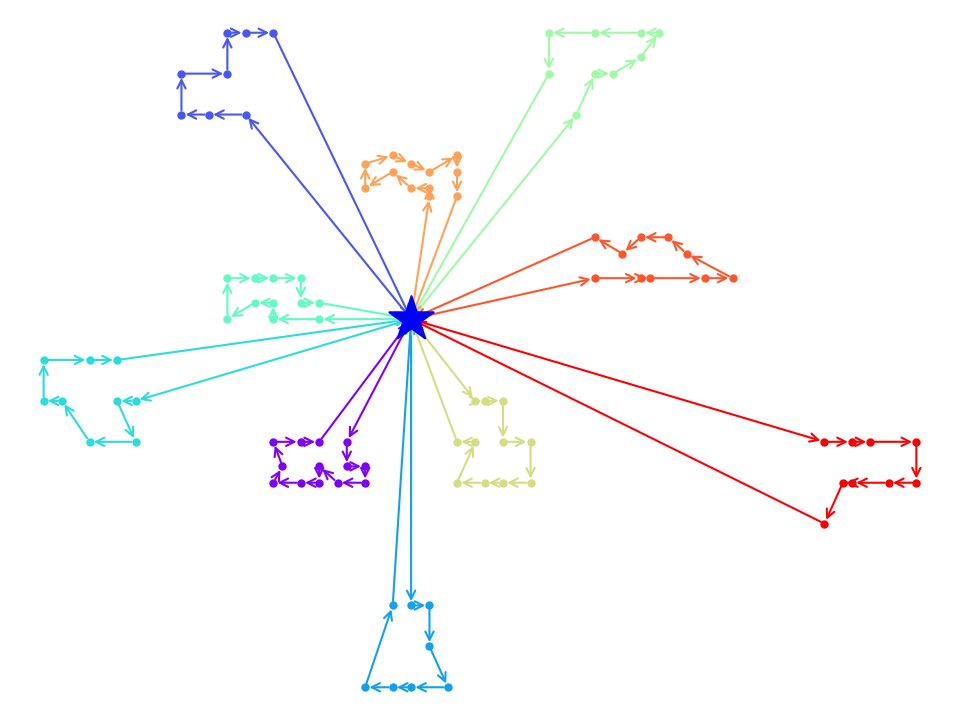
\includegraphics[width=0.3\linewidth]{figures/routes_c101.png}}\quad
    \subfloat[Lớp R]{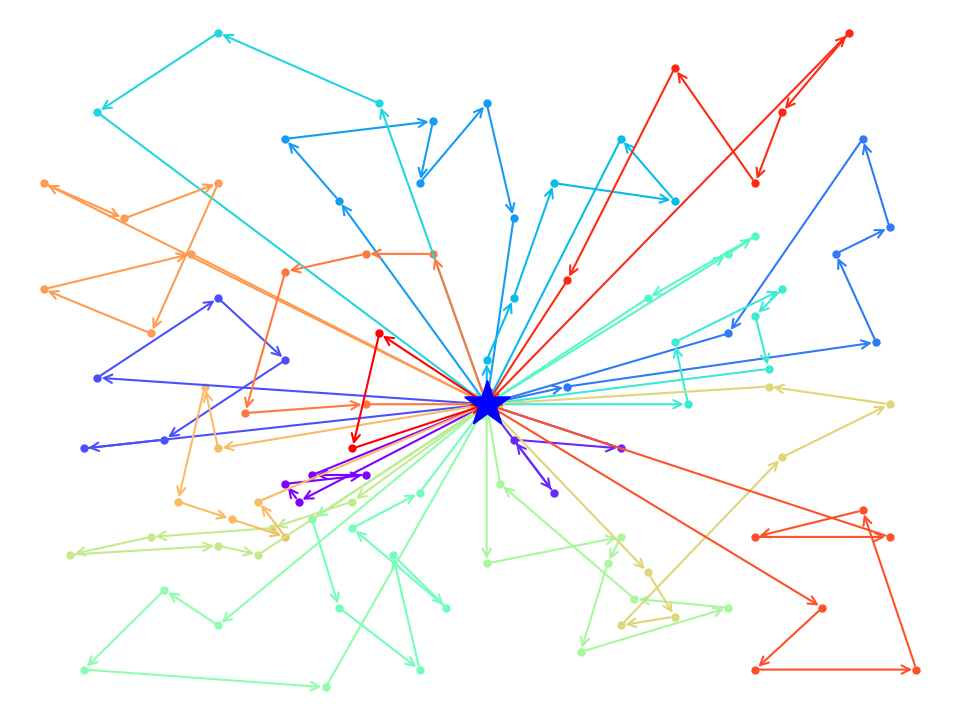
\includegraphics[width=0.3\linewidth]{figures/routes_r101.png}}\quad
    \subfloat[Lớp RC]{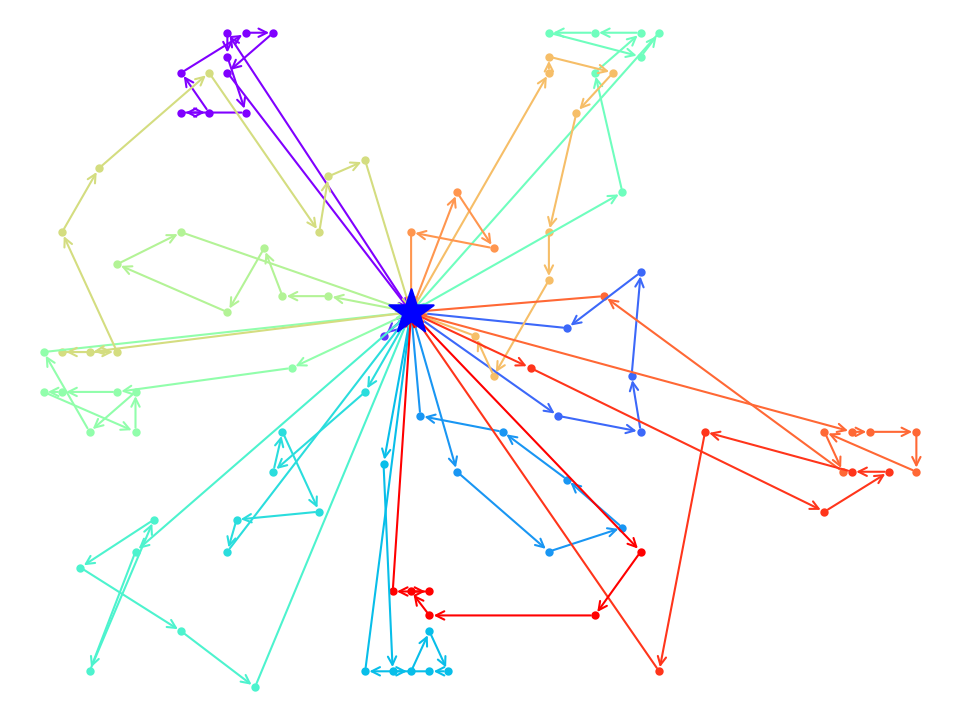
\includegraphics[width=0.3\linewidth]{figures/routes_rc101.png}}
    \caption{Minh họa lời giải cho các lớp cấu hình}
  \end{figure}
\end{frame}